\chapter{Theoretical Prequisites}
The main measurement principle by a \gls{gmr}-Sensor has been already described and characterized exhaustively by \citet{lit:thes:helou}, \citet{lit:thes:reisbeck} and \citet{lit:thes:brenner}. Therefore, this theoretical part will focus on (bio-)physical aspects of a cell rolling motion inside a microfluidic channel and surface modification chemistry.

\section{Microfluidics}
The main experiments of this work were carried out in microfluidic environments, which exhibit favorable properties compared to common turbulent systems. From a fluid-mechanical standpoint, shrinking the scales makes interfacial as well as electrokinetic phenomena much more significant, and reduces the importance of pressure and gravity.\cite{lit:fluidic:kirby} However, electodynamics, chemistry and fluid dynamics are incetricably intertwined, so that fluid flow can create electric fields (and vice versa), with a degree of coupling driven by the surface chemistry. Many of the resulting phenomena arise or can explained by Cauchy-Momentum equation (eq. \ref{eq:cauchymomentum}) and the resulting Navier-Stokes equation for incompressible fluids (eq. \ref{eq:navierstokes}).

\begin{align}
	\frac{\partial}{\partial t} \iiint \rho \mathrm{dV} &= - \iint \rho \mathbf{u} \cdot \vv{\mathbf{n}} \mathrm{dA} \\
	\nabla \cdot \mathbf{u} &= 0 \\
		\rho \frac{\partial \mathbf{u}}{\partial t} + \rho\mathbf{u} \cdot \nabla \mathbf{u} &= \nabla \cdot \boldsymbol{\tau} + \sum_{i}\mathbf{f}_i \label{eq:cauchymomentum} \\	
	\aunderbrace{\vphantom{\sum_{i}} \rho \frac{\partial \mathbf{u}}{\partial t}}_{\mathrm{Transient}} + \aunderbrace{\vphantom{\sum_{i}}\rho\mathbf{u} \cdot \nabla \mathbf{u}}_{\mathrm{Convection}} &= \aunderbrace{\vphantom{\sum_{i}}-\nabla p}_{\mathrm{Pressure}} + \aunderbrace{\vphantom{\sum_{i}}\eta \nabla^2 \mathbf{u}}_{\mathrm{Viscous}} + \aunderbrace{\sum_{i}\mathbf{f}_i}_{\mathrm{Body \ Forces}} \label{eq:navierstokes}
\end{align}
conservation of mass, momentum
reynolds number
\subsection{Flow Field inside Microchannels}
The foremost characteristic of a microchannel is the laminar flow behavior, which causes deterministic pathlines. Mathematically this is described by the reynolds number, which compares the intertia to shear forces. If it results below a certain threshold of 2000, laminar flow can be assumed. This holds true for the utilized microfluidic with the dimensions \SI{12000}{\micro\meter} x \SI{700}{\micro\meter} x \SI{150}{\micro\meter} (l x w x h) and aequous buffer solutions, where the channel width was used as characteristic length $l$. Hence, the Navier-Stokes equation can be applied to our system. 
\begin{equation}
	\mathit{Re}\ =\ \frac{2 \rho |\overline{u}| l }{\eta}
\end{equation}
The step from the Cauchy momentum equation to the Navier-Stokes equation is complex and harbors several sources of error. First, an incompressible newtonian fluid as well as channel is assumed. The used water suspensions can be approximated with negligible compressibility, which is not true for the real case. Also, for blood or other shear-thinning fluids some deviations are prone for high errors. This happens due to the fact that the \acrfull{tau} is decomposed into pressure and viscous contributions as shown in the equations \ref{eq:surfaceStressTensor}. Then, the divergence relation  of the respective viscous stress (eq. \ref{eq:divergence_Stresstensor}) does not hold for non-uniform viscosity $\eta$.
\begin{align}
	\boldsymbol{\tau} &= \boldsymbol{\tau}_{viscous} +  \boldsymbol{\tau}_{pressure} = 2\eta\epsilon - p \mathbf{I}_{\scaleto{3 \times 3}{4pt}} \label{eq:surfaceStressTensor}\\
	\nabla \cdot \boldsymbol{\tau}_{viscous} &= \nabla \cdot 2\eta\epsilon = \nabla \cdot \eta \nabla \mathbf{u} \ \underset{uniform}{\overset{only \ if \ \eta}{=}} \ \eta \nabla^2 \mathbf{u} 	\label{eq:divergence_Stresstensor}
\end{align}
Second, the channel height varies in reality as a result of fabrication inaccuracies. In the model case of a flow through a rectangular channel, no analytical solution of the Navier-Stokes equation exists, but a Fourier Series expansion if channel width is larger than channel height. \cite{lit:fluidic:bruus} The equation \ref{eq:flowVelocityRect} shows that height deviations can have prominent influence on a channel velocity simulation as it is proportional to $h^2$. Further, the flow rate (which is the velocity integral over the channel cross section) depends even on $h^3$. 
\begin{align}
 u   _x(y,z) = \frac{4 h^2 \Delta p}{\pi^3 \eta l} \sum_{n,odd}^{\infty} \frac{1}{n^3} \left( 1- \frac{\cosh (n \pi \frac{y}{h})}{\cosh (n \pi \frac{w}{2h})} \right) \sin (n \pi \frac{z}{h}) \label{eq:flowVelocityRect}
\end{align}
Third, the transient term (eq. \ref{eq:navierstokes}) was neglected in all simulations, but a connected syringe pump possesses a slow rise time (Fig. \ref{fig:fluidic:pumpStability:transient}) and a remaining ``pulsation error'' in steady state (Fig. \ref{fig:fluidic:pumpStability:steadystate}). In effect, another error adds to the simulation, which is only valid after several ten seconds of the last flow rate change.

\begin{figure}
	\begin{subfigure}[b]{0.5\textwidth}
		\centering
	    \addtocounter{subfigure}{1}  
		\subfigimg[clip,trim=115 100 80 60, height=100pt]{a} {./Ressources/Fluidic/Transient_SyringePump.jpg}		
		\addtocounter{subfigure}{-1}  
		\phantomsubcaption
		\label{fig:fluidic:pumpStability:transient}
	\end{subfigure}%
	\begin{subfigure}[b]{0.5\textwidth}
		\centering
		\addtocounter{subfigure}{1}  
		\subfigimg[height=100pt]{\textbf{b}}{./Ressources/Fluidic/SyringeSteadyState.eps}
		\addtocounter{subfigure}{-1}  
		\phantomsubcaption
		\label{fig:fluidic:pumpStability:steadystate}
	\end{subfigure}
\capption{Syringe Pump error sources}{Set flow rate: \orangeMLline, Real Flow Rate: \blueMLline \subref{fig:fluidic:pumpStability:transient} Transient step answer of a syringe pump through a microtube with \SI{254}{\micro\meter} inner diameter. \subref{fig:fluidic:pumpStability:steadystate} Steady state flow rate error around the desired \SI{5}{\micro\liter\per\minute} dispensing rate. A sinusoidal behaviour caused by the microstepping can be observed. \cite{lit:fluidic:fluigentPumpStability}}
\label{fig:fluidic:pumpStability}
\end{figure}

For later studies in a matlab model, the flow velocity and shear stress computations were carried out with the error sources considered. 



\subsection{Particles in Microfluidics}
Stokes Drag Force
Gravity
Electro-static interaction
Magnetic Force
Friction
Interface-Forces
\subsection{}

\section{Surface Chemistry}
Molecules can be immobilized through various mechanisms on surfaces to achieve a biological or chemical functionality. The most simple is physisorption. Here, a biomolecule is bonded only by weak elektrostatic, van-der-Waals or dipole-dipole interaction with a adsorption enthalpy below \SI{50}{\kilo\joule\per\mole}. In contrast, this yields fast reaction rates, because no activation energy has to be overcome. Although a large number of molecules can be captured with this method, several drawbacks have been identified. \cite{lit:bio:ImmobilizationTechniques, lit:bio:immobilization:UV-ABs}
For example, immobilized receptors can start to desorb or change their position, which in turn reduces sensitivity or causes false-positive results. \cite{lit:bio:physisorp:desorption, lit:chem:surfModOptics} \\
Therfore, most functionalization approaches rely on chemisorption where molecules are covalent bound to a surface. Due to the higher activation energy barrier this bonding mechanism works slower in comparison to physisorption though higher temperatures or catalysators can promote an equilibrium. One of the most well-known strategies to achieve reproducible thin films on surfaces is the formation of \glspl{sam} 

\cite{lit:chem:sin:langeDiss}


Weiterhin kann es zu Verschiebungen der adsorbierten Rezeptoren kommen, wodurch es zu falsch-positiven Ergebnissen kommen kann.[9] Daher basieren die meisten Funktionalisierungsmethoden nicht auf der Physisorption, sondern auf der Chemisorption. Hierbei werden Moleküle kovalent an die Oberfläche gebunden. Aufgrund der dabei zu überwindenden Aktivierungsbarriere läuft diese Reaktion langsamer im Vergleich zur Physisorption ab. Bei erhöhten Temperaturen kann das Einstellen des Gleichgewichtes jedoch begünstigt werden. Eine der bekanntesten Strategien dünne Filme auf Oberflächen zu erzeugen, ist die Bildung von selbstorganisierenden Monoschichten (SAM),[46-48] wobei eine kovalente, sehr stabile Bindung zwischen den organischen Komponenten und dem Substrat ausgebildet wird.[49] SAM bilden sich spontan beim Eintauchen in oberflächenaktive Lösungen. Hierzu gehören die Bindung von Alkanthiolen auf Goldoberflächen und die Bindung von Silanen auf Siliziumoberflächen (Abbildung 6).

\subsection{Silane Chemistry}

By the use of silane chemistry a surface is rendered organofunctional with alkoxysilane molecules. Since glass, silicon, alumina, titania, and quartz surfaces, as well as other metal oxide interfaces, are rich in hydroxyl groups, silanes are particularly useful for modifying these materials. These groups attack and displace the alkoxy groups on the silane thus forming a covalent \ch{- Si - O - Si -} bond. \cite{lit:chem:silanizingGlass}

A silane molecule contains a central silicon atom bonded to two types of groups - alkoxy groups and organo-functional groups. These two types exhibit different reactivity allowing sequential reactions and have the ability to form a durable bond between organic and inorganic materials.
The final result of reacting an organosilane with a substrate ranges from altering the wetting or adhesion characteristics of the substrate, utilizing the substrate to catalyze chemical transformation at the heterogeneous interface, ordering the interfacial region, and modifying its partition characteristics. Significantly, it includes the ability to effect a covalent bond between organic and inorganic materials. Especially in optical or biological sensors, silane modifications open a broad range of applications. \cite{lit:chem:GELEST}

Die Einführung von neuen Funktionalitäten durch die Silanisierung der Oberfläche hat eine große Bedeutung in der Biosensorik. Die Hydroxylgruppen können hierbei durch die Reinigung der Oberfläche mit Piranha-Lösung oder UV/Ozon aufgebaut werden kann. Die so erzeugten reaktiven Hydroxylgruppen reagieren anschließend in einer Kondensationsreaktion mit dem Silan (Abbildung 7). Häufig beschrieben wird die Umsetzung von Glasoberflächen oder Siliziumoberflächen mit
3-Aminopropyltrimethoxysilan (APTMS) oder Aminopropyltriethoxysilan (APTES). 

Unterschiede bei der Verwendung von APTES und APTMS liegen in der Reaktivität der Verbindungen. Aufgrund der großen Reaktivität von APTMS werden die Reaktionen in reinen organischen Lösungsmitteln durchgeführt. Dadurch lassen sich dünnere und kontrollierte Schichten mit Aminopropylgruppen erzeugen. Bei der Bildung von Monoschichten mit APTES muss die Reaktion mit Wasser katalysiert werden.[51] Weiterhin wird in der Literatur beschrieben, dass es zu Reaktionen zwischen den Aminogruppen des Silans und den Hydroxylgruppen der Oberfläche kommen kann, wobei keine geordnete Schicht erhalten muss die Reaktion mit Wasser katalysiert werden.[51] Weiterhin wird in der Literatur beschrieben, dass es zu Reaktionen zwischen den Aminogruppen des Silans und den Hydroxylgruppen der Oberfläche kommen kann, wobei keine geordnete Schicht erhalten

\subsubsection{Oxidation}

\begin{figure}[htb!]
%\begin{wrapfigure}[10]{l}{4cm}
	\centering
	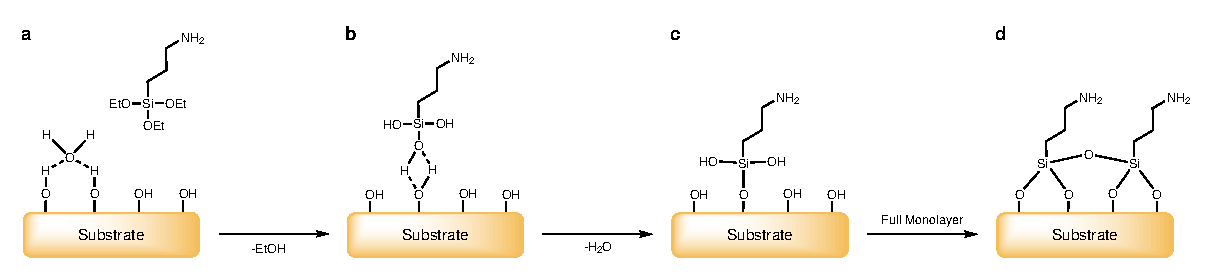
\includegraphics[width=1\linewidth]{./Ressources/Chemistry/APTES.eps}
	\caption{APTES}
	\label{fig:chem:APTES}
%\end{wrapfigure}
\end{figure}
\begin{figure}[htb!]
	\centering
	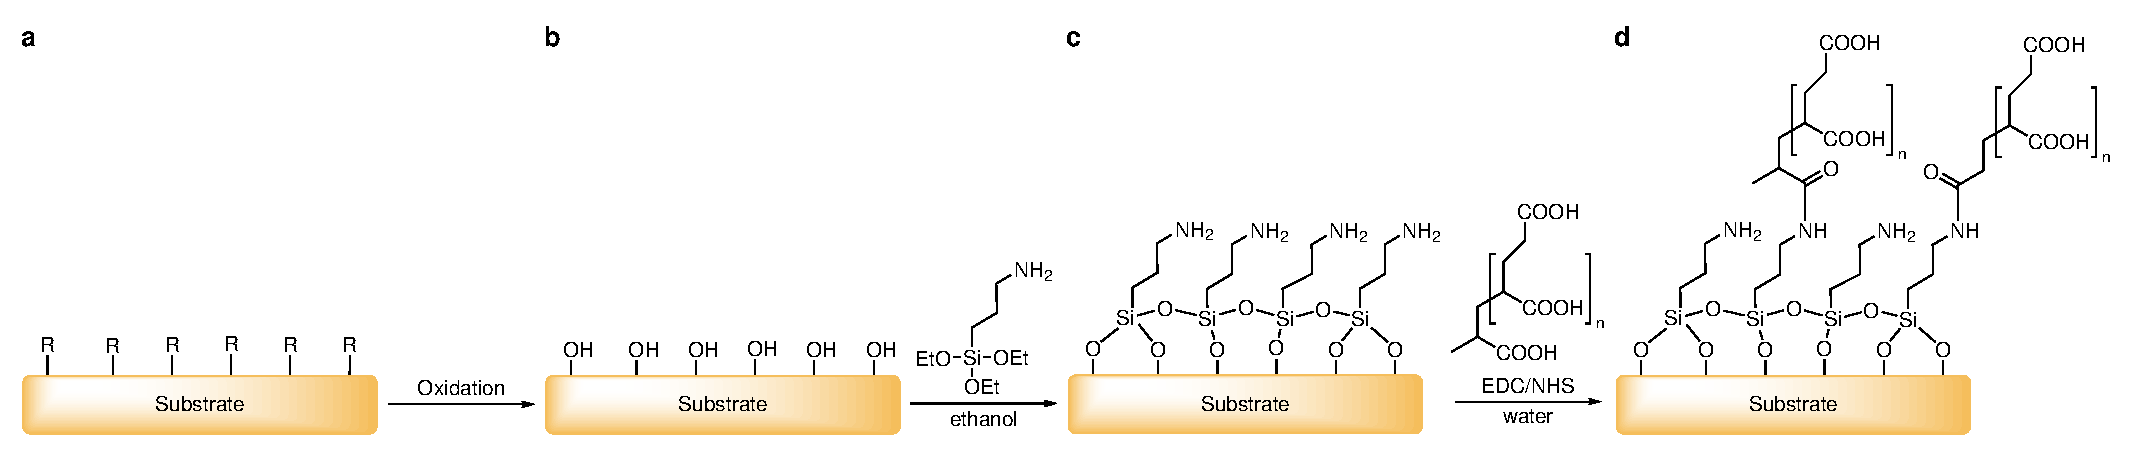
\includegraphics[width=1\linewidth]{Ressources/Chemistry/Substrate}
	\caption{}
	\label{fig:chem:func:substrate}
\end{figure}


\begin{figure}[htb!]
	\begin{subfigure}[b]{0.30\textwidth}
	\centering
	\addtocounter{subfigure}{1}  
	\subfigimg[clip,trim=0 0 0 -40, width=\linewidth]{a} {./Ressources/Chemistry/Glass}		
	\addtocounter{subfigure}{-1}  
	\phantomsubcaption
	\label{fig:chem:func:glass}
\end{subfigure}%
\hfill
\begin{subfigure}[b]{0.69\textwidth}
	\centering
	\addtocounter{subfigure}{1}  
	\subfigimg[clip, trim=0 0 575 120,width=\linewidth]{\textbf{b}}{Ressources/Chemistry/PDMS}
	\addtocounter{subfigure}{-1}  
	\phantomsubcaption
	\label{fig:chem:func:pdms}
\end{subfigure}
\end{figure}
\lipsum[2]
\begin{wrapfigure}[13]{r}{.5\linewidth}
	\centering
	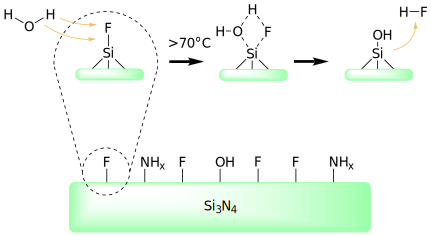
\includegraphics[width=1\linewidth]{Ressources/Chemistry/SiN}
	\capption{\Acrlong{sin} etching with \acrlong{hf}}{}
	\label{fig:chem:func:sin}
\end{wrapfigure}
\lipsum[2]

\subsection{Carbodiimide Crosslinker Chemistry}
EDC-NHS-Activation
sulfo-NHS vs. NHS
\begin{figure}[htb!]
\centering
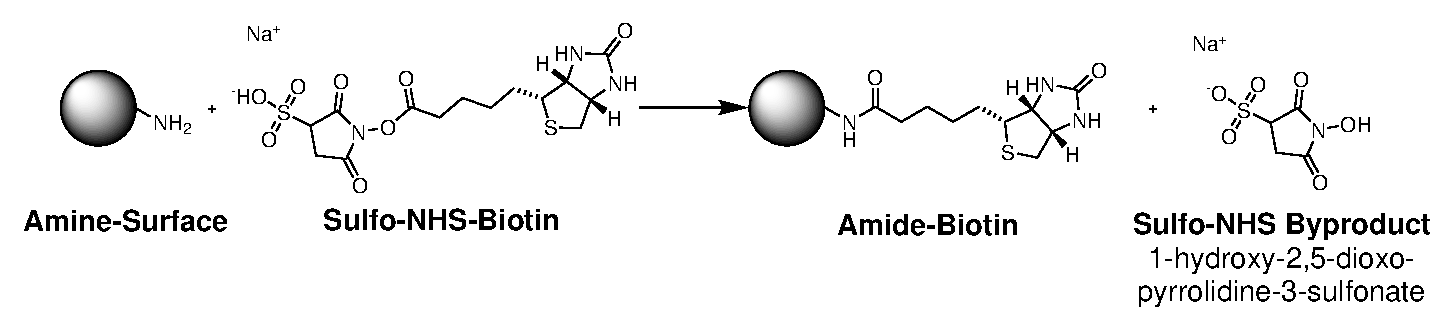
\includegraphics[width=\textwidth]{./Ressources/Chemistry/Sulfo-NHS.eps}
\caption{TestSvg}
\label{fig:Chem:NH2-NHS}
\end{figure}

\begin{figure}[htb!]
\centering
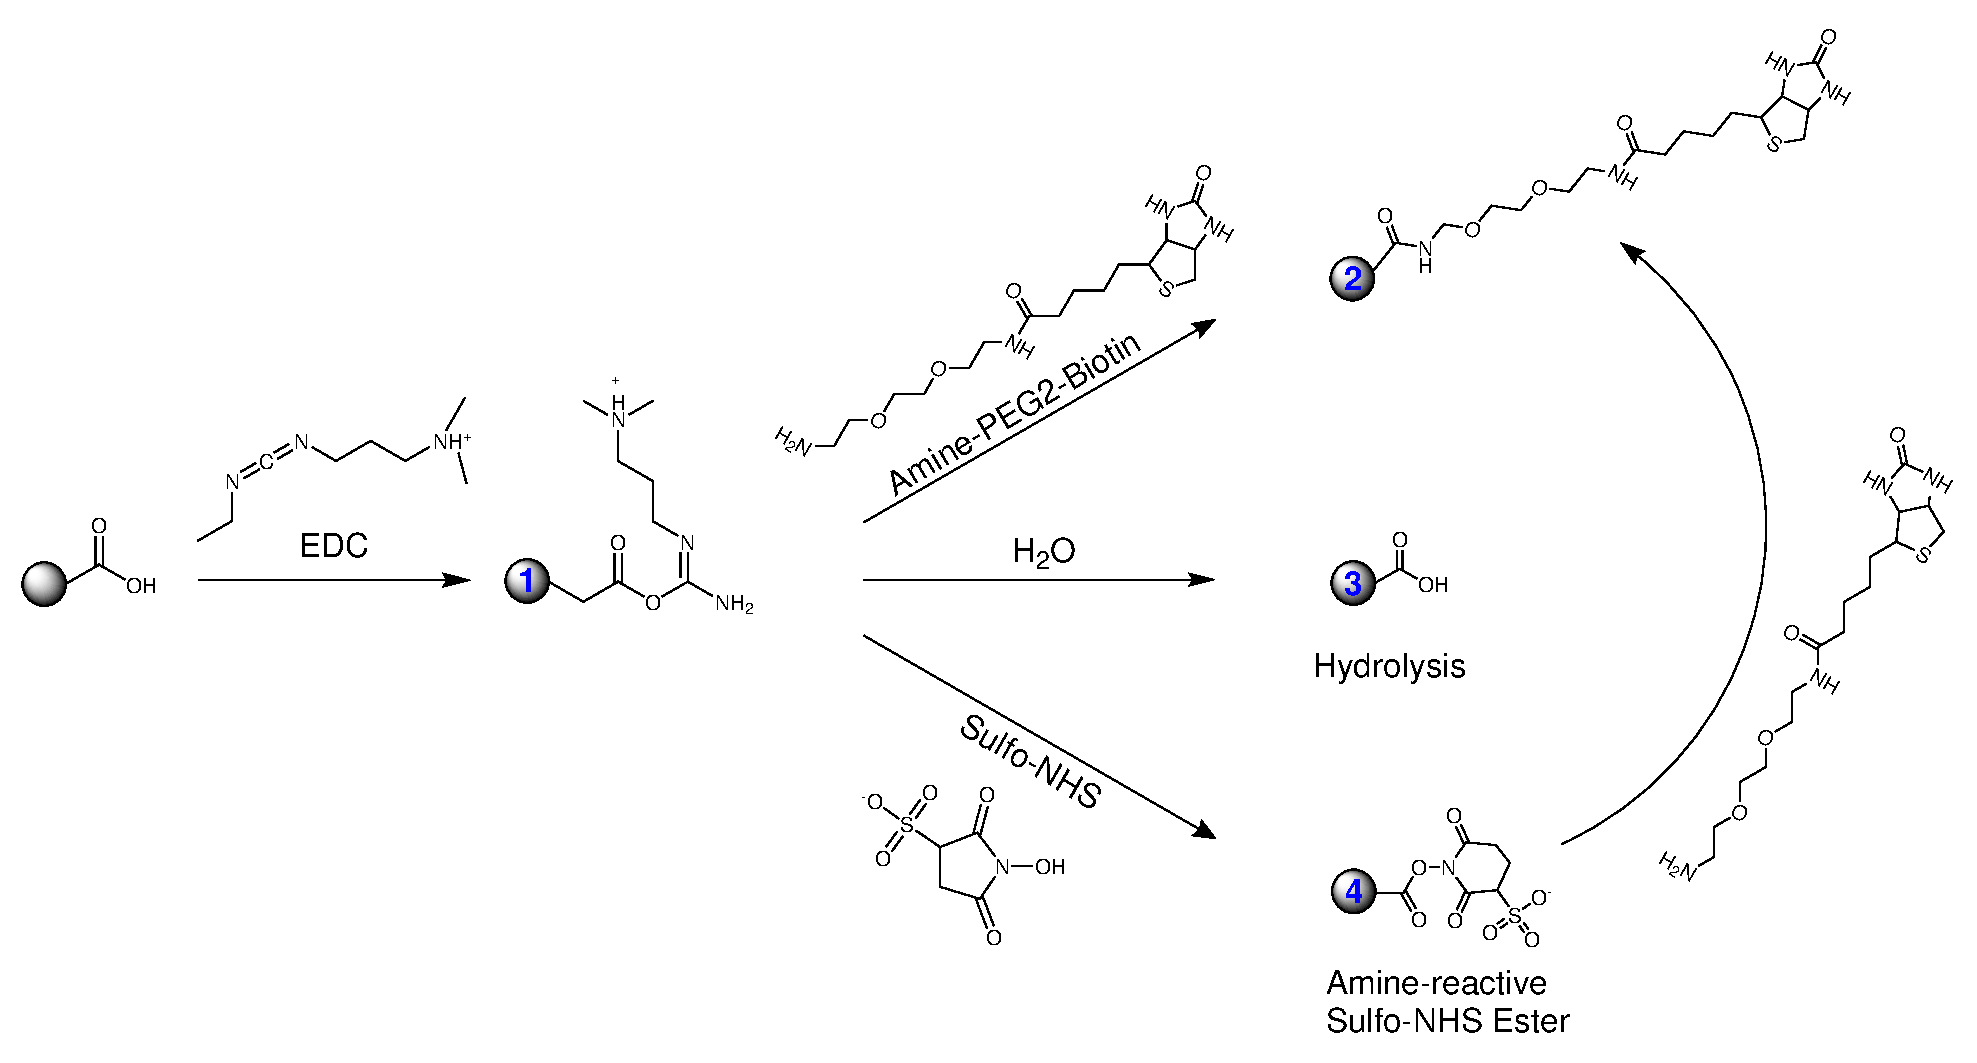
\includegraphics[width=\textwidth]{./Ressources/Chemistry/EDC-NHS.eps}
\capption{TestSvg}{}
\label{fig:Chem:COOH-EDC-NHS}
\end{figure}
\subsection{Microscopic Particle Surface Physics}

\subsection{The Biotin-Avidin-System}


\section{MRCyte}
Short intro over MRCyte
Foto of setup with arrows to necessary parts
Microscope
Stages
PEEK holder
Helmholtz coils
Kepco
MFLI
DAQ
\subsection{Focusing Structures}
test,test
Loss because of reduced velocity and magnetic drag
\subsection{GMR}
Different produced GMR stacks
Wheatstone Bridge setup
Magnet alignment
\subsection{Electrical Circuit}
Ground
PCB
Stacked PCBs with spacer
\subsection{Electronic Readout}
test,test
\subsubsection{Hysteresis Alignment}
test,test
\subsubsection{Single GMR}
test,test
\subsubsection{Dual GMR}
one MFLI supplies both at same freuqency. Aux Trigger tested, but no advantage.


